\chapter{Problema dei cammini minimi - Floyd-Warshall}
Come al solito diamo qualche definizione per poter lavorare successivamente in maniera
agile.
\section{Definizioni}
\subsection{Grafo}
Un Grafo viene definito come $G=(V,E)$ dove:
\begin{itemize}
    \item $V = \{v_1,v_2,v_3,...,v_n\}$ insieme di vertici
    \item $E= \{e_1,e_2,e_3,...,e_m\}$ insieme di archi
\end{itemize}
\paragraph*{Dimensione di G} $\rightarrow$ (n,m).
Arco $e_k \rightarrow$ relazione R tra due vertici $v_i$ e $v_j$
\paragraph*{R può essere}
\begin{itemize}
    \item Simmetrica - Grafo NON Orientato - cioè $v_i \, R \, v_j \Leftrightarrow v_j \, R \, v_i$
    \item Asimmetrica - Grafo Orientato (o diretto) - cioè $v_i \, R \, v_j \nLeftrightarrow  v_j \, R \, v_i$
\end{itemize}
Un grafo orientato è caratterizzato da un verso di percorrenza degli archi unidirezionale.
In questo caso E è sottoinsieme di $V^2$.
\begin{center}
    \includegraphics[width=80mm, scale=0.5]{grafo_orientato.png}
\end{center}
\begin{center}
    \includegraphics[width=80mm, scale=0.5]{grafo_non_orientato.png}
\end{center}
\subsection{Adiacenza}
Un vertifica v è adiacente a un vertice u se $(u,v)\in E$.\\
Per esempio nella rappresentazione del grafo orientato il vertice \textbf{1} è adiacante ai
vertici \textbf{2 e 5}, infatti notiamo che in E è presente $(1,2), (1,5)$.
\subsection{Rappresentazione di un grafo}
Abbiamo 2 rappresentazioni possibili:
\begin{itemize}
    \item Liste di adiacenza
    \item Matrice di adiacenza
\end{itemize}
\begin{enumerate}
    \item Le liste di adiacenza utilizzano un vettore $L_v$ di dimensione $|V|$ tale che $V[i]$ è la lista degli
    adiacenti del vertice $v_i$. Ogni vertice del grafo avrà un vettore.
    \item La matrice di adiacenza è una Matrice $M_v$ di dimensione $n \times n$ tale che $M[i,j] = 1$ se il
    vertice j è adiacente del vertice i, altrimenti $M[i,j] = 0$. A differenza delle liste in questo caso ho una sola
    matrice.
\end{enumerate}
\subsection{Esempio grafo orientato}
\begin{center}
    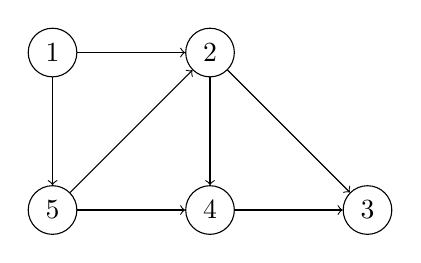
\begin{tikzpicture}
        \node[shape=circle,draw=black] (1) at (0,0) {1};
        \node[shape=circle,draw=black] (2) at (2,0) {2};
        \node[shape=circle,draw=black] (3) at (4,-2) {3};
        \node[shape=circle,draw=black] (4) at (2,-2) {4};
        \node[shape=circle,draw=black] (5) at (0,-2) {5};

        \path [->] (1) edge node[left] {} (2);
        \path [->] (2) edge node[left] {} (3);
        \path [->] (1) edge node[left] {} (5);
        \path [->] (5) edge node[left] {} (2);
        \path [->] (2) edge node[left] {} (4);
        \path [->] (5) edge node[left] {} (4);
        \path [->] (4) edge node[left] {} (3);

    \end{tikzpicture}
\end{center}

\begin{equation*}
    M = \begin{array}{c|ccccc}
    & 1 & 2 & 3 & 4 & 5 \\
    \hline
    1 & 1 & 0 & 0 & 1 & 0 \\
    2 & 0 & 0 & 1 & 1 & 0 \\
    3 & 0 & 0 & 0 & 0 & 0 \\
    4 & 0 & 1 & 0 & 0 & 0 \\
    5 & 1 & 0 & 1 & 0 & 0 \\
    \end{array}
\end{equation*}
\paragraph*{Dimensione} $|V|^2=n^2$
\paragraph*{Numero di celle con 1} $|E|$

\subsection{Esempio grafo non orientato}
\begin{center}
    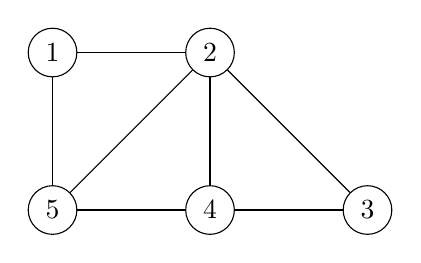
\begin{tikzpicture}
        \node[shape=circle,draw=black] (1) at (0,0) {1};
        \node[shape=circle,draw=black] (2) at (2,0) {2};
        \node[shape=circle,draw=black] (3) at (4,-2) {3};
        \node[shape=circle,draw=black] (4) at (2,-2) {4};
        \node[shape=circle,draw=black] (5) at (0,-2) {5};

        \path [-] (1) edge node[left] {} (2);
        \path [-] (2) edge node[left] {} (3);
        \path [-] (1) edge node[left] {} (5);
        \path [-] (5) edge node[left] {} (2);
        \path [-] (4) edge node[left] {} (2);
        \path [-] (5) edge node[left] {} (4);
        \path [-] (4) edge node[left] {} (3);

    \end{tikzpicture}
\end{center}

\begin{center}
    \begin{equation*}
        M = \begin{array}{c|ccccc}
          & 1 & 2 & 3 & 4 & 5 \\
        \hline
        1 & 0 & 1 & 0 & 0 & 1 \\
        2 & 1 & 0 & 1 & 1 & 1 \\
        3 & 0 & 1 & 0 & 1 & 0 \\
        4 & 0 & 1 & 1 & 0 & 1 \\
        5 & 1 & 1 & 0 & 1 & 0 \\
        \end{array}
        \end{equation*}
\end{center}
\paragraph*{Dimensione} $|V|^2=n^2$
\paragraph*{Numero di celle con 1} $2|E|$
\subsection{Liste VS Matrice (memoria)}
\paragraph*{Liste di adiacenza} Sono ottime dal punto di vista dell'occupazione dello spazio 
nel caso di Grafi sparsi con $|E|$ molto minore di $|V|^2$.
\paragraph*{Matrici di adiacenza} Risultano migliori nei grafi densi quindi quando ho
$|E|$ che si avvicina a $|V|^2$.
\subsection{Liste VS Matrice (tempo)}
\paragraph*{(u,v)} Intendiamo se i 2 vertici sono collegati.
Come tempo intendiamo il tempo per stabilire se (u,v) appartiene ad E e i tempi
sono i seguenti:
\begin{itemize}
    \item Liste di adiacenza $\rightarrow O(|E|) = O(m)$
    \item Matrice di adiacenza $\rightarrow O(1)$
\end{itemize}
\subsection{Cammino in un grafo orientato}
\paragraph*{Definizione di cammino} Sequenza $P=<v_{i_1},v_{i_2},..., v_{i_{k-1}},v_{i_k}>$
tale che $v_{i_k}$ appartiene a V per $1\leq j \leq k$ e $(v_{i_j},v_{i_{j+1}})$ appartiene
ad E per $1 \leq j < k$.
\paragraph*{Lunghezza del cammino} $k-1$ (numero di archi)
\paragraph*{Ciclo} Cammino in cui $v_{i_1}$ coincide con $v_{i_k}$
\paragraph*{Cammino semplice} Cammino in cui ogni vertice è presente una volta sola (cioè non
contiene cicli)
\paragraph*{Predecessore di $v_{i_k}$ in P} Vertice di $v_{i_{k-1}}$
\subsection{Grafo orientato pesato}
\paragraph*{Grafo} $G = (V,E,W)$
\begin{itemize}
    \item $V = \{v_1,v_2,v_3,...,v_n\}$ insieme di vertici
    \item $E= \{e_1,e_2,e_3,...,e_m\}$ insieme di archi
    \item $W:E \rightarrow R$ tale che $W(v_i,v_j) = w_{ij}$ è il peso dell'arco
    $(v_i,v_j)$
\end{itemize}
\paragraph*{Peso di un cammino} Si tratta della somma dei pesi di tutti gli
archi, formalmente: $P=<v_{i_1},v_{i_2},...,v_{i_k}> \rightarrow \sum^{k-1}_{j=1}w(v_{i_j},v_{i_{j+1}})$
\subsection{Esempio grafo orientato pesato}
\begin{center}
    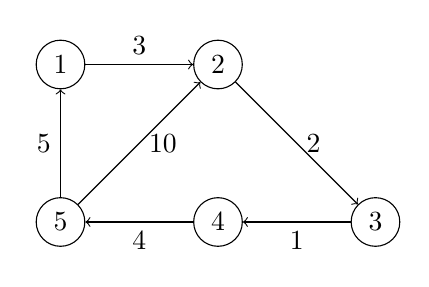
\begin{tikzpicture}
        \node[shape=circle,draw=black] (1) at (0,0) {1};
        \node[shape=circle,draw=black] (2) at (2,0) {2};
        \node[shape=circle,draw=black] (3) at (4,-2) {3};
        \node[shape=circle,draw=black] (4) at (2,-2) {4};
        \node[shape=circle,draw=black] (5) at (0,-2) {5};
    
        \path [->] (1) edge node[midway, above] {3} (2);
        \path [->] (2) edge node[midway, right] {2} (3);
        \path [->] (3) edge node[midway, below] {1} (4);
        \path [->] (4) edge node[midway, below] {4} (5);
        \path [->] (5) edge node[midway, left] {5} (1);
        \path [->] (5) edge node[midway, right] {10} (2);
        
    \end{tikzpicture}
\end{center}
\section{Il problema dei cammini minimi - Algoritmo di Floyd-Warshall}
Floyd-Warshall è un algoritmo che sfruttra la programmazione dinamica per calcolare i cammini minimi fra tutte le coppie
in un grafo orientato $G = (V,E)$. Ha un tempo di esecuzione di $\Theta(V^3)$.\\
Floyd-Warshall accetta in input grafi contenenti archi di peso negativo, ma si suppone non ci siano cicli di peso negativo.
\paragraph*{Input} Grafo $G=(V,E,W)$ (senza cappi) orientato e pesato
\paragraph*{Output} Per ogni coppia di vertici i e j, trovare il cammino di peso minimo (cammino minimo)
che parte da i e finisce in j.\\
Si tratta di un problema di ottimizzazione di minimo, dove
\begin{itemize}
    \item (n) $\rightarrow$ dimensione del problema
    \item Soluzioni possibili per una coppia di vertici i e j sono tutti i cammini da i a j
    \item Funzione obiettivo è il peso del cammino
    \item Peso del cammino minimo da i a j è il valore ottimi (per i e j)
    \item Un cammino minimo tra i vertici i e j è la soluzione ottimale
\end{itemize}
\subsection{L'input}
\paragraph*{Funzione peso W} $W:E \rightarrow R^+$ tale che $W(i,j) = w_{ij} =$ peso dell'arco $(i,j)$.
\paragraph*{Funzione peso W - Versione estesa} $W:V \times V \rightarrow R^+$ tale che $W(i,j) = w_{ij}$ con:
\begin{itemize}
    \item $w_{ij} = 0$ se $i=j$
    \item $w_{ij} =$ peso dell'arco $(i,j)$, se $(i,j) \in E$
    \item $w_{ij} = \infty$, se $i \neq j$ e $(i,j) \notin E$ 
\end{itemize}
Matrice $W=[w_{ij}]$ di n righe e n colonne.
\subsection{L'output Matrici D e $\Pi$}
\begin{itemize}
    \item Matrice $D = [d_{ij}]$ di n righe e n colonne, dove $ [d_{ij}]$ è il peso del
    cammino minimo da i e j
    \item Matrice $\Pi = [\pi_{ij}]$ di n righe e n colonne, dove $\pi_{ij}$ è il predecessore di j
    nel cammino minimo da i a j
\end{itemize}
\paragraph*{Matrice D}
\begin{itemize}
    \item $d_{ij} = 0$ se $i = j$
    \item $d_{ij} = $ peso del cammino minimo, se esiste un cammino da i a j
    \item $d_{ij} = \infty$ se non esiste un cammino da i a j
\end{itemize}
\paragraph*{Matrice $\Pi$}
\begin{itemize}
    \item $\pi_{ij} = NIL$, se $i = j$
    \item $\pi_{ij} = u$ appartenente al cammino minimo da i a j, tale che $(u,j) \in E$, se
    esiste un cammino da i a j
    \item $\pi_{ij} = NIL$, se non esisto un cammino da i a j
\end{itemize}
Dopo aver riempito entrambe le matrici mi rendo conto che:\\
\textbf{La riga i d $\Pi$ fornisce l'albero dei predecessori relativo al vertice i}.
\paragraph{Albero dei predecessori del vertice i (riga i di $\Pi$)}
\begin{itemize}
    \item $\{ j \in V | \pi_{ij} \notin NIL\} \cup \{i\} \rightarrow$ insieme dei vertici
    \item ${(\pi_{ij}, j) | \pi{ij} \notin NIL}$
\end{itemize}
\section{Sosttostruttura ottima (primo tentativo)}
Consideriamo come $P_{ij}$ il \textbf{Cammino minimo da i a j} e p è il predecessore di j.\\
Sicuramente $P_{ij} = P_{ip} + <j>$, con $P_{ip}$ cammino minimo da i a p.
\begin{center}
    \includegraphics[width=70mm, scale=0.5]{chapters_ulerich/img/floyd_warshall_tent_sottostruttura.png}
\end{center}
Con $P_{ip}$ cammino minimo da i a p. Come potrei trovare $P_{ij}$?
\begin{center}
    \includegraphics[width=70mm, scale=0.5]{chapters_ulerich/img/floyd_warshall_tent_sottostruttura_2.png}
\end{center}
\begin{enumerate}
    \item Considero tutti i vertici p' tali che $(p',j) \in E$
    \item Per ogni vertice p' determino il cammino dato da: $P_{ip} + <j>$
    \item Seleziono il cammino di peso minimo
\end{enumerate}
\paragraph*{Attenzione!} Non è sicuro che quando si calcola $P_{ij}$ si abbiano già a disposizione
i cammini $P_{ip'}$.
Si deve parametrizzare rispetto alla lunghezza I del cammino:
\begin{enumerate}
    \item Prima calcolo tutti i cammini minimi a lunghezza $0 \rightarrow P^0_{ij}$\\
    $P^0_{ij} = <i>$ se $i = j$, altrimenti $P^0_{ij} = \infty$
    \item Poi calcolo tutti i cammini minimi a lunghezza 1 $\rightarrow P^1_{ij}$\\
    $P^1_{ij} = <i,j>$ se $i \neq j$ e $(i,j) \in E$, altrimenti $P^1_{ij} = \infty$
    \item Poi calcolo tutti i cammini minimi a lunghezza 2 $\rightarrow P^2_{ij}$
    \item Poi calcolo tutti i cammini minimi a lunghezza 3 $\rightarrow P^3_{ij}$
    \item ...
    \item Ci si ferma per $l = |E| = m$ (l è lunghezza)
    \item Per ogni coppia i e j scelgo tra i cammini $P^0_{ij}, P^1_{ij}, \dots, P^m_{ij}$,
    quello di peso minimo
\end{enumerate}
\paragraph*{Friendly Reminder} $<i,j>$ Significa perorso con i vertici i e j.
\paragraph*{Domande} Come calcolo $P^l_{ij}$ con $l \geq 2$?\\
E qual è il tempo nel caso peggiore dell'algoritmo DP che sfrutta questa struttura ottima?\\
\subsection{Diamo un ordine ai vertici del grafo}
1 viene prima di 2 che viene prima di 3 etc. che viene prima dell'ultimo vertice n.\\
Parametriziamo rispetto ai vertici intermedi del cammino:
\begin{itemize}
    \item Trovo $P^0_{ij} \rightarrow$ cammino minimo senza vertici intermedi
    \item Trovo $P^1_{ij} \rightarrow$ cammino minimo con vertici intermedi $\in \{1\}$
    \item Trovo $P^2_{ij} \rightarrow$ cammino minimo con vertici intermedi $\in \{1,2\}$
    \item Trovo $P^3_{ij} \rightarrow$ cammino minimo con vertici intermedi $\in \{1,2,3\}$
    \item Trovo $P^n_{ij} \rightarrow$ cammino minimo con vertici intermedi $\in \{1,2,\dots,n\}$
\end{itemize}
\subsection*{Analizziamo nel dettaglio i cammini minimi intermedi}
$P^0_{ij} \rightarrow$ cammino minimo senza vertici intermedi.
\begin{align*}
  &P^0_{ij} = <i> \quad \text{se} \, i=j \\
  &P^0_{ij} = <i,j> \quad \text{se} \, i \neq j \text{ e } (i,j) \in E \\
  &P^0_{ij} = NIL \quad \text{se} \, i \neq j \text{ e } (i,j) \notin E
\end{align*}
Per $k > 0$, $P^k_{ij} \rightarrow$ cammino minimo con vertici intermedi $\in \{1,2,\dots,k\}$.\\
Per $k = n$, $P^n_{ij} \rightarrow$ cammino minimo con vertici intermedi $\in \{1,2,\dots,n\}$.\\
Quindi $P^n_{ij} \rightarrow$ cammino minimo $P_{ik}$.\\
\paragraph*{Sottoproblema di dimensione k} Per ogni coppia (i,j), trovare il cammino minimo
$P^k_{ij}$ dal vertice i al vertice j che ha vertici intermedi $\in \{1,2,\dots,k\}$ se $k>0$,
oppure non ha vertici intermedi se $k=0$.\\
\begin{align*}
    &k \in \{0,1,\dots,n\}\\
    &i \in \{1,\dots,n\}\\
    &j \in \{1,\dots,n\}
\end{align*}
\textbf{Numero di sottoproblemi} $n\times n \times (n+1)$.\\
$k = n \rightarrow P^n_{ij} = P_{ij}$.
\subsection{Equazioni di ricorrenza}
\paragraph*{Casi base} Sottoproblema di dimensione (0)
\begin{align*}
    &P^0_{ij} = <i> \quad \text{se } i = j\\
    &P^0_{ij} = <i, j> \quad \text{se } i \neq j \text{ e } (i,j) \in E\\
    &P^0_{ij} = NIL \quad \text{se } i \neq j \text{ e } (i,j) \notin E
\end{align*}
\paragraph*{Passo ricorsivo} Tutti i sottoproblemi di dimensione (k) tale che $k > 0$
\begin{align*}
    P^k_{ij} = ?
\end{align*}
Ricerchiamo la sottostruttura ottima.\\
\begin{center}
    \includegraphics[width=70mm, scale=0.5]{chapters_ulerich/img/floyd_warshall_tent_sottostruttura_3.png}
\end{center}
\textbf{Data una soluzione ottimale $P_{ij}=P^n_{ij}$ si possono verificare due casi:}
\begin{enumerate}
    \item Il vertice n NON è uno dei vertici intermedi
    \item Il vertice n è uno dei vertici intermedi
\end{enumerate}
\subsection*{Caso 1 - Il vertice n NON è uno dei vertici intermedi}
\begin{itemize}
    \item $P^n_{ij}$ coincide con $P^{n-1}_{ij}$
    \item Predecessore di j in $P^n_{ij}$ coincide con predecesore di j in $P^{n-1}_{ij}$
\end{itemize}
\subsection*{Caso 2 - Il vertice n è uno dei vertici intermedi}
\begin{align*}
    P^n_{ij} = P_1 + P_2
\end{align*}
\begin{center}
    \includegraphics[width=70mm, scale=0.5]{chapters_ulerich/img/floyd_warshall_tent_sottostruttura_4.png}
\end{center}
\begin{align*}
    P_1 = P^{n-1}_{in} \rightarrow P^n_{ij} = P_1 + P_2 = P^{n-1}_{in} + P_2
\end{align*}
Mentre per quanto riguarda $P_2$ avrò che
\begin{align*}
    P_2 = P^{n-1}_{nj}
\end{align*}
Quindi sostituendo $P_2$ all'interno dell'equazione avrò che:
\begin{align*}
    P_2 = P^{n-1}_{nj} \rightarrow P^n_{ij} = P_1 + P_2 = P^{n-1}_{in} + P^{n-1}_{nj}
\end{align*}
Abbiamo quindi che il predecessore di j in $P^n_{ij}$ coincide con il predecessore di j in $P^{n-1}_{nj}$.\\
\subsection*{Passo ricorsivo per $P^n_{ij}$}
La soluzione ottimale $P^n_{ij} = P_{ij}$ è data da:
\[ P^n_{ij} = min_p\{P^{n-1}_{ij}, P^{n-1}_{in} + P^{n-1}_{nj}\} \]
$i = n$ oppure $j = n \rightarrow \, P^n_{ij} = P^{n-1}_{ij}$.
\subsection*{Passo ricorsivo per $P^k_{ij}$}
La soluzione ottimale $P^k_{ij} (k>0)$ è data da:
\begin{align*}
    P^k_{ij} = min_p{P^{k-1}_{ij}, P^{k-1}{ik} + P^{k-1}_{kj}}
\end{align*}
$i=k$ oppure $j=k \rightarrow \, P^k_{ij} = P^{k-1}_{ij}$.
\subsection{Equazioni di ricorrenza}
Riassumendo abbiamo le sequenti equazioni di ricorrenza:
\paragraph*{k=0 (CASI BASE)}
\begin{align*}
    &P^0_{ij} = <i> \quad \text{se } i = j\\
    &P^0_{ij} = <i, j> \quad \text{se } i \neq j \text{ e } (i,j) \in E\\
    &P^0_{ij} = NIL \quad \text{se } i \neq j \text{ e } (i,j) \notin E
\end{align*}
\paragraph*{$k>0$ (PASSO RICORSIVO)}
\begin{align*}
    P^k_{ij} = min_p{P^{k-1}_{ij}, P^{k-1}{ik} + P^{k-1}_{kj}}
\end{align*}
\subsection*{Definizione dei coefficienti}
\textbf{Coefficienti $d^k_{ij}$ dei sottoproblemi}.\\
$d^k_{ij} \rightarrow$ peso del cammino $P^k_{ij}$
\begin{align*}
    &k \in \{0,1,\dots,n\}\\
    &i \in \{1, \dots, n\}\\
    &j \in \{1,...,n\}
\end{align*}
Quindi abbiamo \textbf{Numero di coefficienti} uguale a $n \times n \times (n+1)$.\\
$k=n \rightarrow d^n_{ij}$ è il preso $d_{ij}$ di $P_{ij}$.\\
Ricordiamo che la funzione obiettivo è trovare il peso del cammino, definiamo quindi i
coefficienti nella seguente maniera:
\paragraph*{k=0 (CASI BASE)}
\begin{align*}
    &d^0_{ij} = 0 \quad \text{se } i = j\\
    &d^0_{ij} = w_{ij} \quad \text{se } i \neq j \text{ e } (i,j) \in E\\
    &d^0_{ij} = \infty \quad \text{se } i \neq j \text{ e } (i,j) \notin E
\end{align*}
\paragraph*{$k>0$ (PASSO RICORSIVO)}
\begin{align*}
    d^k_{ij} = min_p{d^{k-1}_{ij}, d^{k-1}{ik} + d^{k-1}_{kj}}
\end{align*}
\subsection*{Predecessori $\pi^k_{ij}$}
$\pi^k_{ij} \rightarrow$ predecessore del vertice j in $P^k_{ij}$
\begin{align*}
    &k \in \{0,1,\dots,n\}\\
    &i \in \{1, \dots, n\}\\
    &j \in \{1,...,n\}
\end{align*}
\textbf{Numero di predecessori}:: $n \times n \times (n+1)$.\\
$\pi^n_{ij} \rightarrow $ predecessore $\pi_{ij}$ di j in $P_{ij}$.\\
Aggiungiamo alle equazioni di ricorrenza anche i predecessori.
\paragraph*{k=0 (CASI BASE)}
\begin{align*}
    &d^0_{ij} = 0 \quad \pi^0_{ij} = NIL \quad \text{se } i = j\\
    &d^0_{ij} = w_{ij} \quad \pi^0_{ij} = i \quad \text{se } i \neq j \text{ e } (i,j) \in E\\
    &d^0_{ij} = \infty \quad \pi^0_{ij}= NIL \quad \text{se } i \neq j \text{ e } (i,j) \notin E
\end{align*}
\paragraph*{$k>0$ (PASSO RICORSIVO)}
\begin{align*}
    &d^k_{ij} = min_p{d^{k-1}_{ij}, d^{k-1}{ik} + d^{k-1}_{kj}}\\
    &\pi^k_{ij} = \pi^{k-1}_{ij} \text{ se } d^k_{ij} = d^{k-1}_{ij} \text{ altrimenti } 
    \pi^k_{ij} = \pi^{k-1}_{kj}
\end{align*}
\section{Algoritmo bottom-up}
Per ogni valore di k da 0 a n, vengono calcolate due matrici $(n\times n)$:
\begin{align*}
    &D^k=[d^k_{ij}]\\
    &\Pi^k=[\pi^k_{ij}]
\end{align*}
Il numero totale di matrici è $2(n+1)$.
\paragraph*{Caso Base} Ho che:
\begin{align*}
    &D^0=[d^0_{ij}] = W \text{ matrice dei pesi input}\\
    &\Pi^0=[\pi^0_{ij}]
\end{align*}
\paragraph*{Passo Ricorsivo} In questo caso ho:
\begin{align*}
    &D^k=[d^k_{ij}] \text{ e } \Pi^k=[\pi^k_{ij}]\\
    &\text{ Sono calcolate usando le matrici } D^{k-1} = [d^{k-1}_{ij}] \text{ e }
    \Pi^{k-1} = [\pi^{k-1}_{ij}]
\end{align*}
Avrò quindi che le matrici $D^n = [d^n_{ij}]$ e $\Pi^n = [\pi^n_{ij}]$ sono le matrici di
output!
\subsection{Algoritmo bottom-up - Codice}
\begin{lstlisting}[language=Java, escapeinside={*@}{@*}]
    Procedura calcola_valori_ottimi_FW(V,E,W)
      *@$D^0$@* = W
      *@$\Pi^0$@* = (n x n) matrix of NIL values
      for i = 1 to n do
        for j = 1 to n do
         if i != j and *@ $w_{ij}$ != $\infty$@* then
            *@ $\Pi^0$@* [i,j] = i
      for k = 1 to n do
        for i = 1 to n do
            for j = 1 to n do
                *@$D^k[i,j] = D^{k-1}[i,j]$@*
                *@$\Pi^k[i,j] = \Pi^{k-1}[i,j]$@*
                if i != k and j != k then
                    if *@$D^k[i,j]>D^{k-1}[i,k] + D^{k-1}[k,j]$@* then
                        *@$D^k[i,j] = D^{k-1}[i,k]+ D^{k-1}[k,j]$@*
                        *@$\Pi^k[i,j] = \Pi^{k-1}[k,j]$@*
\end{lstlisting}
\paragraph*{Tempo} $\Theta(n^3)$.
\subsubsection*{Rappresentazione esecuzione algoritmo}
Link al video \href{https://www.youtube.com/watch?v=4OQeCuLYj-4&ab_channel=MichaelSambol}{Youtube}.